\documentclass{beamer}
\usepackage{beamerthemesplit}
\usepackage{wrapfig}
\usetheme{SPbGU}
\usepackage{pdfpages}
\usepackage{amsmath}
\usepackage{cmap} 
\usepackage[T2A]{fontenc} 
\usepackage[utf8]{inputenc}
\usepackage[english,russian]{babel}
\usepackage{indentfirst}
\usepackage{amsmath}
\usepackage{tikz}
\usepackage{multirow}
\usepackage[noend]{algpseudocode}
\usepackage{algorithm}
\usepackage{algorithmicx}
\usetikzlibrary{shapes,arrows}
\usepackage{fancyvrb}
%\usepackage{minted}
%\usepackage{verbments}


\newtheorem{rutheorem}{Теорема}
\newtheorem{ruproof}{Доказательство}
\newtheorem{rudefinition}{Определение}
\newtheorem{rulemma}{Лемма}
\beamertemplatenavigationsymbolsempty

\title[]{Синтаксический анализ для поиска в метагеномных сборках}
%\subtitle[YaccConstructor]{Использование вторичной структуры}
% То, что в квадратных скобках, отображается в левом нижнем углу. 
\institute[]{
Лаборатория языковых инструментов JetBrains \\
Санкт-Петербургский государственный университет \\
Математико-механический факультет }

% То, что в квадратных скобках, отображается в левом нижнем углу.
\author[Семён Григорьев]{Семён Григорьев}

\date{11 мая 2016г.}

\definecolor{orange}{RGB}{179,36,31}

\begin{document}
{
\begin{frame}[fragile]
  \begin{tabular}{p{2.5cm} p{5.5cm} p{2cm}}
   \begin{center}
      \includegraphics[width=2cm]{pictures/JBLogo3.pdf}
    \end{center}
    &
    \begin{center}
      \includegraphics[width=1.5cm]{pictures/SPbGU_Logo.png}
    \end{center}
    &
    \begin{center}
      \includegraphics[width=1cm]{pictures/YC_big.jpg}
    \end{center} 
  \end{tabular}
  \titlepage
\end{frame}
}

\begin{frame}[fragile]
  \transwipe[direction=90]
  \frametitle{YaccConstructor}
  \begin{itemize}
    \item Исследования в области лексического и синтаксического анализа
    \item Открытый исходный код
    \begin{itemize}
      \item \url{https://github.com/YaccConstructor}
    \end{itemize}
    \item Основной язык разработки --- F\#
  \end{itemize}
\end{frame}

\begin{frame}
  \transwipe[direction=90]
  \frametitle{Обзор}
  \begin{itemize}
    \item  
  \end{itemize}
\end{frame}


\begin{frame}[fragile]
\transwipe[direction=90]
\frametitle{Динамически формируемый код}

\begin{tabular}{p{4.5cm} p{8cm}}
\begin{minipage}[t]{4cm}
\begin{Verbatim}[commandchars=\\\{\}]
\textcolor{blue}{string} res = \textcolor{orange}{""};
\textcolor{blue}{for}(i = 0; i < l; i++)
    res = \textcolor{orange}{"()"} + res;
\fbox{\textcolor{blue}{use}(res);}

\end{Verbatim}

%\hrule
Аппроксимация
\begin{Verbatim}[commandchars=\\\{\}]
(\textcolor{orange}{"()"})*
\end{Verbatim} 

%\includegraphics[width=2cm]{../../../2015/PSI/slides/pictures/lex1}

\includegraphics[width=3cm]{../../../2015/PSI/slides/pictures/in31}

Грамматика\\
\vspace{-5pt}
$$
\begin{array}{crcl}
&start &::=& s \\
&s & ::= & \mbox{\texttt{LBR }} s \mbox{\texttt{ RBR }} s\\
&s & ::= &\epsilon
\end{array}
$$
\end{minipage}

&

\begin{minipage}[t]{8cm}
Лес разбора ({\bfseries{SPPF}}) \\
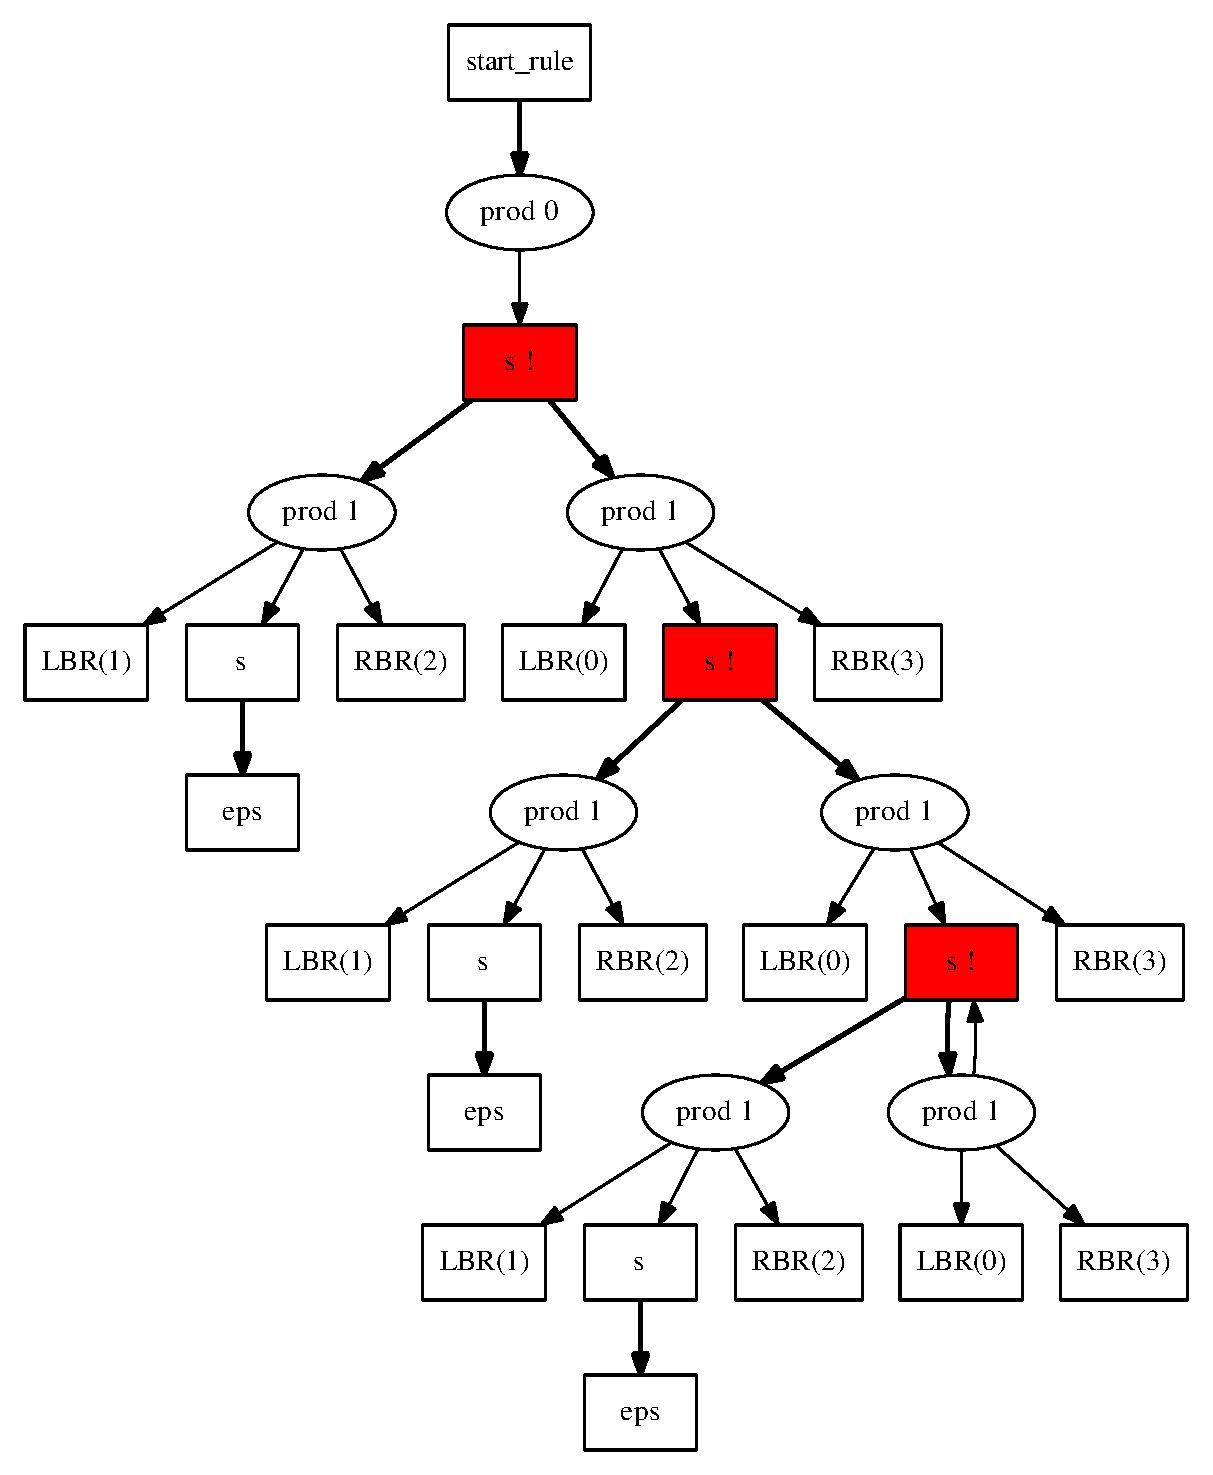
\includegraphics[width=7cm]{../../../2015/PSI/slides/pictures/out3}
\end{minipage}

\end{tabular}

\end{frame}

\begin{frame}[fragile]
  \transwipe[direction=90]
  \frametitle{Задача: применение анализа строковых выражений для JavaScript eval}
  \begin{itemize}
    \item Цель: трансляция стандартного \texttt{eval} в "безопасный"
    \begin{itemize}
        \item Martin Lester. Information Flow Analysis for a Dynamically Typed Functional Language with Staged Metaprogramming
        \item Martin Lester. Analysing Eval using Staged Metaprogramming
    \end{itemize} 
    \item Исследовательская задача: диплом, публикации
    \item Разбивается на 2 подзадачи
    \begin{itemize}
        \item Получение аппроксимации
        \item Трансляция SPPF в "безопасный \texttt{eval}"        
    \end{itemize} 
  \end{itemize}
\end{frame}

\begin{frame}
  \transwipe[direction=90]
  \frametitle{Задача: использование SPPF в абстрактном синтаксическом анализе}
  \begin{itemize}
    \item Абстрактный синтаксический анализ --- один из подходов к анализу динамически формируемого кода
    \begin{itemize}
        \item K. G. Doh, H. Kim, D. A. Schmidt. Static Validation of Dynamically Generated HTML Documents Based on Abstract Parsing and Semantic Processing
        \item \href{https://github.com/YaccConstructor/articles/blob/master/2015/PSI/paper/psi_2015.pdf}{E. Verbitskaia, S. Grigorev, D. Avdyukhin. Relaxed Parsing of Regular Approximations of String-Embedded Languages}
    \end{itemize} 
    \item Реализовать вычисление семантики по статьям
    \item Сравнить с нашим подходом
    \item А можно ли использовать SPPF
    \item Диплом, публикации
  \end{itemize}
\end{frame}

\begin{frame}[plain,c]
 \transwipe[direction=90]
 \begin{center}
  \Huge Средства для сертификацонного программирования \\ или \\ $F\# + F^* = \, ?$
 \end{center}
\end{frame}

\begin{frame}[fragile]
  \transwipe[direction=90]
  \frametitle{Сертификационное программирование}
%  \begin{tabular}[t]{p{6cm} p{8cm}}
  \begin{itemize}
    \item \underline{\bfseries{$F^*$} (\url{https://www.fstar-lang.org/tutorial/})}
    \item Coq
    \item Agda
    \item ...
  \end{itemize}


%\end{tabular}
\end{frame}


\begin{frame}
  \transwipe[direction=90]
  \frametitle{Задача: объединение $F\#$ и $F^*$}
  \begin{itemize}
    \item $F\# + F^* = F\#^*$
    \item Парсер для $F\#^*$
    \item Транслятор из AST $F\#$ в AST $F^*$
    \item Разбивается на подзадачи (до 3 человек)
    \item Диплом (вся задача), публикации
  \end{itemize}
\end{frame}

\begin{frame}
  \transwipe[direction=90]
  \frametitle{Задача: поддержка $F\#^*$ в Microsoft Visual Studio}
  \begin{itemize}
    \item Поддержать в модели проекта, редакторе, отладчике
      \begin{itemize}
        \item Создание файлов, шаблоны
        \item Подсветка синтаксиса
        \item Сообщения об ошибках, подсветка ошибок
        \item ....
      \end{itemize}
    \item Разбивается на подзадачи (до 4 человек)
    \item Диплом (вся задача), публикации
  \end{itemize}
\end{frame}

\begin{frame}
  \transwipe[direction=90]
  \frametitle{Задача: межъязыковое взаимодействие $F\#$ и $F^*$}
  \begin{itemize}
    \item Использовать функции, написанные на $F^*$ в $F\#$(.NET)
    \item Использовать функции, написанные на $F\#$(.NET) в $F^*$
    \item Сохранить типизацию/вывод типов
    \item Разбивается на подзадачи (до 2 человек)
    \item Диплом (вся задача), публикации
  \end{itemize}
\end{frame}
            
\begin{frame}
\transwipe[direction=90]
\frametitle{Контакты}
\begin{itemize}
  \item Почта: \url{rsdpisuy@gmail.com}
  \item Исходный код YaccConstructor: \url{https://github.com/YaccConstructor}
  \item Google+ сообщество: \url{https://goo.gl/DuPWkM}
\end{itemize}
\end{frame}
\end{document}
